\documentclass[Rapport/Rapport_main.tex]{subfiles}
\begin{document}
\subsection{BallCountSensor}\label{sec:BallCountSensor}
Denne sensor står for at notificere systemet om, hvorvidt bolddispenseren har brug for flere bolde.

\subsubsection{Hardwaredesign}
Der benyttes et kredsløb med en optisk sensor, som består at en fotodiode og en IR LED. LED'en lyser ned i et rør, og bolde reflekterer lyset. Afhængig af hvor mange bolde der er, reflekteres der mere eller mindre lys. LED'en sættes til at blinke med en frekvens på 400Hz og en dutycycle på 20\%. I 'on' tiden løber der en relativ stor strøm på 300mA. Dette er for, at lysintensiteten er så stor som mulig. Til at styre lyset bruges der en transistor, som kan levere op til 500mA. 

Dernæst designes fotodiodekredsløbet. Her bruges 4 komponenter: En modstand, et 'sample \& hold' kredsløb, en ADC-konverter og en PWM-generator. Ideen er at bruge en modstand til at forstærke et strømsignal om til en spænding, som så kan samples af 'sample \& hold' kredsløbet. Kloksignalet til 'sample \& hold' og LED'en synkroniseres vha. PWM-komponenten. Det samlede kredsløb kan ses på figur \ref{fig:PSoC_TopDesign}.

\begin{figure}[H]
    \centering
    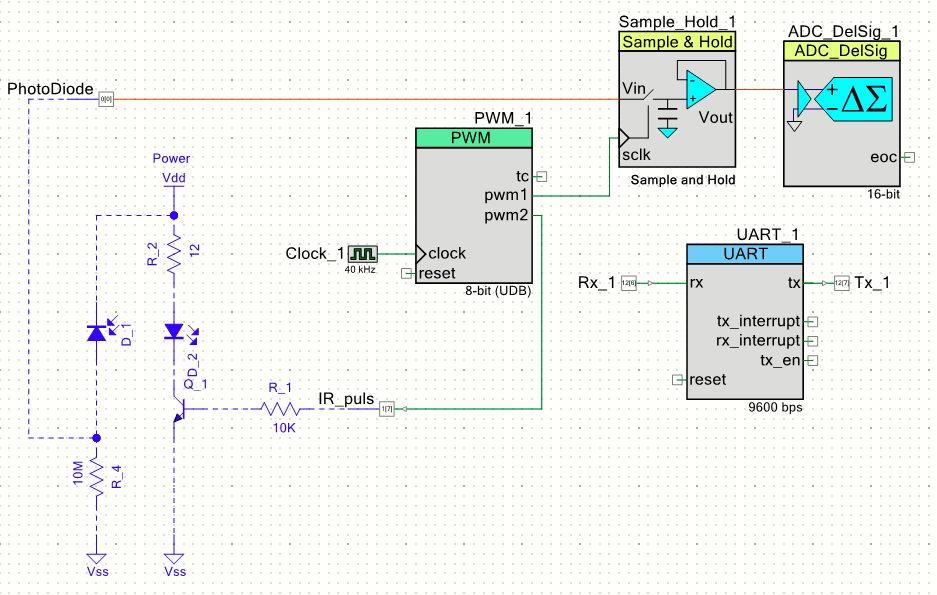
\includegraphics[width=1\textwidth]{Rapport/BallDispenser/BallCountSensor/graphics/Opstilling2.png}
    \caption{Opstilling for Ball Count sensor kredsløb}
    \label{fig:PSoC_TopDesign}
\end{figure}
Til at omregne ADC værdien til hvor mange bolde der er, udføres der en række målinger. I koden for PSoC bruges UART og ADC til at måle værdier alt efter, hvor mange bolde der i cyllinderbeholderen, hvor efter der kodes grænseværdier ind for antallet af bolde.

En tabel over de forskellige grænseværdier kan ses på tabel \ref{table:Treshold_BallCount}
\begin{table}[H]
\centering
\begin{tabular}{|C{0.1\textwidth}|C{0.25\textwidth}|L{0.25\textwidth}|}
\hline 
\textbf{Antal bolde} & \textbf{ADC værdi} & \textbf{status LED's}\\
\hline
1 & 1000 til 14999 & Rød\\
\hline
2 & 15000 til 29999 & Rød\\
\hline
3 & 30000 til 40000 & Slukket\\
\hline
4 & 1 til 400 & Grøn\\
\hline
\end{tabular}
\caption{Grænseværdier for BallCountSensor}
\label{table:Treshold_BallCount}
\end{table}
\end{document}